\documentclass[notheorems,aspectratio=169]{beamer}

\usepackage{ctex}
\usepackage{fontspec}
\usepackage{xeCJK}
\IfFontExistsTF{Noto Serif CJK JP}{
  \setCJKmainfont{Noto Serif CJK JP}
  \setCJKsansfont{Noto Sans CJK JP}
  \setCJKmonofont{Noto Sans Mono CJK JP}
}{
  \IfFontExistsTF{Microsoft YaHei}{
    \setCJKmainfont{Microsoft YaHei}
    \setCJKsansfont{Microsoft YaHei}
  }{}
}
\usepackage{amsmath,amssymb,bm}
\usepackage{booktabs,array}
\usepackage{tikz}
\usetikzlibrary{
  arrows.meta,angles,quotes,calc,positioning,patterns,
  decorations.pathmorphing,shapes.geometric
}

\usetheme{Madrid}
\usefonttheme[onlymath]{serif}
\setbeamertemplate{navigation symbols}{}
\let\Tiny\tiny

\definecolor{ChinaRed}{RGB}{196,30,58}
\definecolor{JapanBlue}{RGB}{0,82,155}
\definecolor{SoftBlue}{RGB}{231,241,249}
\definecolor{SoftRed}{RGB}{252,235,239}
\definecolor{GraphGray}{RGB}{95,105,115}
\definecolor{ForceGreen}{RGB}{22,135,92}
\definecolor{SoftGreen}{RGB}{232,247,240}
\definecolor{ForceGold}{RGB}{218,145,18}

\setbeamercolor{structure}{fg=JapanBlue}
\setbeamercolor{frametitle}{fg=white,bg=JapanBlue}
\setbeamercolor{title}{fg=white,bg=JapanBlue}
\setbeamercolor{block title}{fg=white,bg=JapanBlue}
\setbeamercolor{block body}{fg=black,bg=SoftBlue}
\setbeamercolor{example text}{fg=ForceGreen}
\setbeamercolor{block title example}{fg=white,bg=ForceGreen}
\setbeamercolor{block body example}{fg=black,bg=SoftGreen}
\setbeamercolor{alerted text}{fg=ChinaRed}

\newcommand{\jp}[1]{\textbf{\color{JapanBlue}#1}}
\newcommand{\key}[1]{\textbf{\color{ChinaRed}#1}}
\newcommand{\en}[1]{\textcolor{GraphGray}{\scriptsize(#1)}}
\newcommand{\ans}[1]{\textcolor{ForceGreen}{\textbf{答：}#1}}
\newcommand{\qcard}[1]{%
  \begin{block}{問題}\centering\large #1\end{block}}
\newcommand{\qsmall}[1]{%
  \begin{block}{問題（再掲）}\small #1\end{block}}
\newcommand{\acard}[1]{%
  \begin{exampleblock}{解答・考え方}#1\end{exampleblock}}
\newcommand{\stepbox}[2]{%
  \begin{beamercolorbox}[rounded=true,sep=0.7em,wd=\linewidth]{block body}
  \textbf{\color{JapanBlue}#1}\quad #2
  \end{beamercolorbox}}
\newcommand{\vect}[1]{\bm{#1}}

\title[EJU Physics]{物理4}
\subtitle{剛体のつり合い・ニュートンの三法則・仕事と力学的エネルギー}
\author[Sirui Liu]{Sirui Liu}
\date{2026年7月}

\AtBeginSection[]{
  \begin{frame}[plain]
    \vfill
    \centering
    {\usebeamerfont{title}\color{JapanBlue}\insertsectionhead\par}
    \vspace{0.8em}
    {\color{GraphGray}\large EJU Physics}
    \vfill
  \end{frame}
}

\begin{document}

\begin{frame}
  \titlepage
\end{frame}

\begin{frame}{今日の到達目標}
  \begin{enumerate}
    \item \jp{力のモーメント（力矩）}を用いて、剛体のつり合いを立式できる。
    \item \jp{ニュートンの三法則}を区別し、物体ごとに運動方程式を作れる。
    \item \jp{仕事・仕事率}を、力と変位の向きまで含めて計算できる。
    \item \jp{力学的エネルギー保存則}の成立条件を判断し、運動を解ける。
  \end{enumerate}

  \vfill
  \begin{block}{贯穿全课的一条主线}
    \centering
    \key{研究对象を決める}
    $\longrightarrow$
    \key{図を描く}
    $\longrightarrow$
    \key{法則を選ぶ}
    $\longrightarrow$
    \key{符号と単位を確認する}
  \end{block}
\end{frame}

% ============================================================
\section{剛体・力のモーメント・つり合い}

\begin{frame}{質点と剛体}
  \begin{columns}[T,onlytextwidth]
    \column{0.50\textwidth}
    \begin{block}{質点（しつてん）}
      大きさや回転を無視し、質量が一点に集まったと考える模型。
      \[
        \sum \vect F = m\vect a
      \]
      只关心\key{平动}。
    \end{block}

    \begin{block}{剛体（ごうたい）}
      力を受けても形が変わらない理想物体。平动だけでなく
      \key{回転}も考える。
    \end{block}

    \column{0.46\textwidth}
    \centering
    \begin{tikzpicture}[scale=0.85,>=Latex]
      \fill[JapanBlue] (0,2.5) circle (3pt);
      \draw[->,very thick,ChinaRed] (0,2.5)--(1.7,2.5)
        node[right] {$\vect F$};
      \node[below=3pt] at (0,2.5) {質点};

      \draw[rounded corners,thick,fill=SoftBlue]
        (-1.4,-0.4) rectangle (1.4,0.7);
      \fill[JapanBlue] (0,0.15) circle (2.5pt);
      \draw[->,very thick,ChinaRed] (1.1,0.55)--(2.3,1.35)
        node[right] {$\vect F$};
      \draw[->,thick,ForceGreen] (0.65,0.15) arc (0:230:0.65);
      \node at (0,-0.85) {剛体：平動＋回転};
    \end{tikzpicture}
  \end{columns}
\end{frame}

\begin{frame}{力のモーメント（ちからのモーメント）}
  \begin{columns}[T,onlytextwidth]
    \column{0.49\textwidth}
    \begin{block}{定義 \en{torque / moment}}
      回転軸から力の作用点までの位置ベクトルを $\vect r$、
      力を $\vect F$ とすると
      \[
        \boxed{\tau=rF\sin\theta=Fd}
      \]
      $d$ は回転軸から\key{作用線}までの垂直距離
      \jp{腕の長さ（うでのながさ）}。
    \end{block}
    \[
      [\tau]=\mathrm{N\,m}
    \]
    同じ $\mathrm{N\,m}$ でも、エネルギーの単位 J とは意味が異なる。

    \column{0.47\textwidth}
    \centering
    \begin{tikzpicture}[scale=0.9,>=Latex]
      \coordinate (O) at (0,0);
      \coordinate (P) at (3.3,0);
      \coordinate (Q) at ($(P)+(60:1)$);
      \draw[line width=5pt,GraphGray] (O)--(P);
      \fill[JapanBlue] (O) circle (3pt) node[below] {支点 $O$};
      \draw[->,very thick,ChinaRed] (P)--++(60:2.0)
        node[above] {$\vect F$};
      \draw[->,thick,JapanBlue] (O)--(P)
        node[midway,below] {$r$};
      \draw pic[
        draw=ForceGold,->,angle radius=8mm,
        angle eccentricity=1.35,"$\theta$"
      ]{angle=O--P--Q};
      \draw[dashed,ChinaRed] ($(P)+(-60:1.2)$)--($(P)+(60:2.3)$);
      \draw[densely dashed,ForceGreen] (O)--($(P)+(-60:1.65)$);
      \node[ForceGreen] at (1.55,-1.15) {$d=r\sin\theta$};
    \end{tikzpicture}
  \end{columns}
\end{frame}

\begin{frame}{符号・作用線・支点の選び方}
  \begin{columns}[T,onlytextwidth]
    \column{0.49\textwidth}
    \begin{block}{符号規則}
      通常は
      \[
        \text{反時計回り }(+),\qquad
        \text{時計回り }(-)
      \]
      と決める。相反する约定也可以，但必须全程一致。
    \end{block}

    \begin{alertblock}{ゼロになる場合}
      力の作用線が支点を通ると $d=0$ なので
      \[
        \tau=0.
      \]
      力が大きくても回転効果はない。
    \end{alertblock}

    \column{0.47\textwidth}
    \begin{block}{立式技巧}
      未知力が作用する点を支点に選ぶと、その未知力のモーメントは
      0 になり、式が簡単になる。
    \end{block}
    \centering
    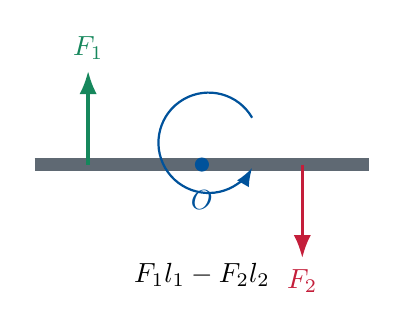
\begin{tikzpicture}[scale=0.85,>=Latex]
      \draw[line width=5pt,GraphGray] (-2.5,0)--(2.5,0);
      \fill[JapanBlue] (0,0) circle (3pt) node[below=6pt] {$O$};
      \draw[->,very thick,ForceGreen] (-1.7,0)--(-1.7,1.4)
        node[above] {$F_1$};
      \draw[->,very thick,ChinaRed] (1.5,0)--(1.5,-1.4)
        node[below] {$F_2$};
      \draw[->,JapanBlue,thick] (0.75,0.7) arc (30:330:0.75);
      \node at (0,-1.65) {$F_1l_1-F_2l_2$};
    \end{tikzpicture}
  \end{columns}
\end{frame}

\begin{frame}{剛体のつり合い条件}
  \begin{block}{静止を続けるための二条件}
    \[
      \boxed{\sum \vect F=\vect 0}
      \qquad\text{かつ}\qquad
      \boxed{\sum \tau_O=0}
    \]
    第一式保证\key{平动平衡}，第二式保证\key{转动平衡}。
  \end{block}

  \begin{columns}[T,onlytextwidth]
    \column{0.48\textwidth}
    \stepbox{1. 物体を孤立させる}{所有外力を描く。}
    \vspace{0.5em}
    \stepbox{2. 軸を決める}{未知力が多い点を優先。}
    \column{0.48\textwidth}
    \stepbox{3. 力の式}{通常は $x,y$ 方向に分ける。}
    \vspace{0.5em}
    \stepbox{4. モーメントの式}{正負と垂直距離を確認。}
  \end{columns}

  \vfill
  \centering
  \key{どの点まわりで計算しても、つり合いなら結果は同じ。}
\end{frame}

\begin{frame}{例題1｜シーソー：問題}
  \vfill
  \qcard{
    質量 $30\,\mathrm{kg}$ の子どもが支点の左 $2.0\,\mathrm{m}$ に座る。
    質量 $40\,\mathrm{kg}$ の子どもは、右側のどこに座れば
    シーソーが水平につり合うか。板の質量は無視する。
  }
  \vfill
\end{frame}

\begin{frame}{例題1｜シーソー：解答}
  \qsmall{
    $30\,\mathrm{kg}$ が左 $2.0\,\mathrm{m}$。右の $40\,\mathrm{kg}$ の位置 $x$ を求める。
  }
  \begin{columns}[T,onlytextwidth]
    \column{0.47\textwidth}
    \centering
    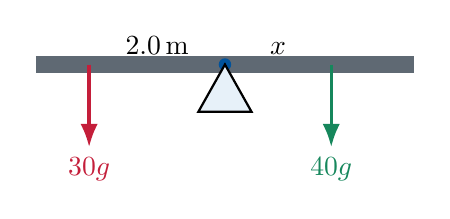
\begin{tikzpicture}[scale=0.75,>=Latex]
      \draw[line width=6pt,GraphGray] (-3.2,0)--(3.2,0);
      \fill[JapanBlue] (0,0) circle (3pt);
      \draw[fill=SoftBlue,thick] (-0.45,-0.8)--(0.45,-0.8)--(0,0)--cycle;
      \draw[->,very thick,ChinaRed] (-2.3,0)--(-2.3,-1.4)
        node[below] {$30g$};
      \draw[->,very thick,ForceGreen] (1.8,0)--(1.8,-1.4)
        node[below] {$40g$};
      \node[above] at (-1.15,0) {$2.0\,\mathrm m$};
      \node[above] at (0.9,0) {$x$};
    \end{tikzpicture}
    \column{0.49\textwidth}
    \acard{
      支点まわりのモーメントをとる。
      \[
        30g\times2.0=40g\times x
      \]
      \[
        x=\frac{30\times2.0}{40}
        =\boxed{1.5\,\mathrm m}
      \]
      \ans{支点の右 $1.5\,\mathrm m$。}
    }
  \end{columns}
\end{frame}

\begin{frame}{例題2｜棒に斜めの力：問題}
  \vfill
  \qcard{
    長さ $0.80\,\mathrm m$ の棒の端に、大きさ $50\,\mathrm N$ の力を
    棒となす角 $30^\circ$ で加える。反時計回りを正とするとき、
    反対側の端を支点とした力のモーメントの大きさを求めよ。
  }
  \vfill
\end{frame}

\begin{frame}{例題2｜棒に斜めの力：解答}
  \qsmall{
    $r=0.80\,\mathrm m$, $F=50\,\mathrm N$, $\theta=30^\circ$。
    モーメントの大きさを求める。
  }
  \begin{columns}[T,onlytextwidth]
    \column{0.48\textwidth}
    \centering
    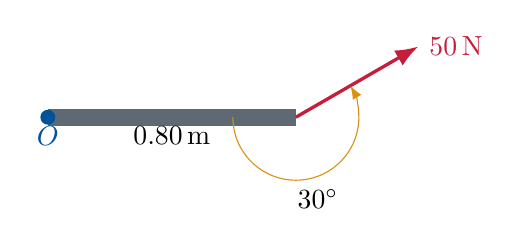
\begin{tikzpicture}[scale=0.9,>=Latex]
      \coordinate (Otwo) at (0,0);
      \coordinate (Ptwo) at (3.5,0);
      \coordinate (Qtwo) at ($(Ptwo)+(30:1)$);
      \draw[line width=6pt,GraphGray] (Otwo)--(Ptwo);
      \fill[JapanBlue] (Otwo) circle (3pt) node[below] {$O$};
      \draw[->,very thick,ChinaRed] (Ptwo)--++(30:2)
        node[right] {$50\,\mathrm N$};
      \draw pic[
        draw=ForceGold,->,angle radius=8mm,
        angle eccentricity=1.35,"$30^\circ$"
      ]{angle=Otwo--Ptwo--Qtwo};
      \node[below] at (1.75,0) {$0.80\,\mathrm m$};
    \end{tikzpicture}
    \column{0.48\textwidth}
    \acard{
      棒に垂直な成分だけが回転に寄与する。
      \[
        \tau=rF\sin\theta
      \]
      \[
        =0.80\times50\times\sin30^\circ
        =\boxed{20\,\mathrm{N\,m}}
      \]
      图中为反時計回り，所以符号为正。
    }
  \end{columns}
\end{frame}

\begin{frame}{重心・支持面・転倒}
  \begin{columns}[T,onlytextwidth]
    \column{0.50\textwidth}
    \begin{block}{重心（じゅうしん）}
      重力が一点に集中して働くとみなせる点。均一な対称物体では、
      通常は幾何学的中心と一致する。
    \end{block}
    \begin{alertblock}{転倒条件}
      重心から鉛直下向きに引いた線が
      \jp{支持面（しじめん）}の外へ出ると、端を支点として
      転倒する。
    \end{alertblock}
    \begin{itemize}
      \item 重心が低いほど安定。
      \item 支持面が広いほど安定。
    \end{itemize}

    \column{0.46\textwidth}
    \centering
    \begin{tikzpicture}[scale=0.85,>=Latex]
      \draw[thick] (-2.5,0)--(2.5,0);
      \draw[fill=SoftBlue,thick,rotate around={12:(0,0)}]
        (-1.1,0) rectangle (1.1,2.2);
      \fill[JapanBlue] (0.23,1.08) circle (3pt)
        node[right] {重心};
      \draw[->,very thick,ChinaRed] (0.23,1.08)--(0.23,-0.2)
        node[below] {$mg$};
      \draw[very thick,ForceGreen] (-1.1,0)--(1.1,0);
      \node[ForceGreen,below=5pt] at (0,0) {支持面};
      \draw[dashed,GraphGray] (1.1,0)--(1.1,2.8);
      \node[align=center] at (0,-1.0)
        {重力の作用線が\\支持面内なら安定};
    \end{tikzpicture}
  \end{columns}
\end{frame}

\begin{frame}{例題3｜一様な棒：問題}
  \vfill
  \qcard{
    長さ $4.0\,\mathrm m$、質量 $20\,\mathrm{kg}$ の一様な水平棒を、
    左端 $A$ と右端 $B$ で支える。左端から $1.0\,\mathrm m$ の位置に
    質量 $40\,\mathrm{kg}$ の物体を置いた。$g=10\,\mathrm{m/s^2}$ として、
    支持力 $N_A,N_B$ を求めよ。
  }
  \vfill
\end{frame}

\begin{frame}{例題3｜一様な棒：解答}
  \qsmall{
    $4.0\,\mathrm m$ の一様棒（$20\,\mathrm{kg}$）に、
    左から $1.0\,\mathrm m$ の位置で $40\,\mathrm{kg}$。
    両端の支持力を求める。
  }
  \begin{columns}[T,onlytextwidth]
    \column{0.50\textwidth}
    \centering
    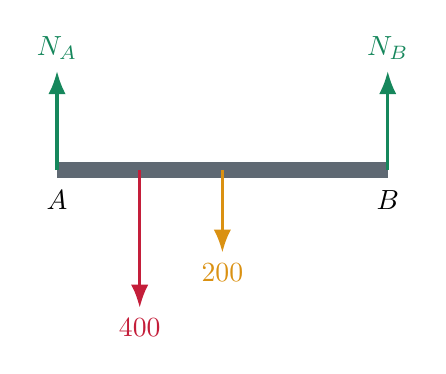
\begin{tikzpicture}[x=1.05cm,y=0.007cm,>=Latex]
      \draw[line width=6pt,GraphGray] (0,0)--(4,0);
      \draw[->,very thick,ForceGreen] (0,0)--(0,180)
        node[above] {$N_A$};
      \draw[->,very thick,ForceGreen] (4,0)--(4,180)
        node[above] {$N_B$};
      \draw[->,very thick,ChinaRed] (1,0)--(1,-250)
        node[below] {$400$};
      \draw[->,very thick,ForceGold] (2,0)--(2,-150)
        node[below] {$200$};
      \node[below=4pt] at (0,0) {$A$};
      \node[below=4pt] at (4,0) {$B$};
    \end{tikzpicture}
    \column{0.46\textwidth}
    \acard{
      $A$ まわり：
      \[
        4N_B-400\times1-200\times2=0
      \]
      よって $N_B=200\,\mathrm N$。
      鉛直方向：
      \[
        N_A+N_B=400+200
      \]
      \[
        \boxed{N_A=400\,\mathrm N,\quad N_B=200\,\mathrm N}
      \]
    }
  \end{columns}
\end{frame}

\begin{frame}{例題4｜箱が転倒する直前：問題}
  \vfill
  \qcard{
    幅 $0.60\,\mathrm m$、高さ $1.20\,\mathrm m$、重さ $300\,\mathrm N$ の
    一様な箱の上端を水平に押す。床との摩擦は十分大きく滑らない。
    箱が転倒し始める水平力 $F$ を求めよ。
  }
  \vfill
\end{frame}

\begin{frame}{例題4｜箱が転倒する直前：解答}
  \qsmall{
    幅 $0.60\,\mathrm m$、高さ $1.20\,\mathrm m$、重さ $300\,\mathrm N$。
    上端を水平に押す。転倒直前の $F$ は？
  }
  \begin{columns}[T,onlytextwidth]
    \column{0.45\textwidth}
    \centering
    \begin{tikzpicture}[scale=1.0,>=Latex]
      \draw[thick] (-0.7,0)--(3.2,0);
      \draw[fill=SoftBlue,thick] (0,0) rectangle (1.5,3);
      \fill[JapanBlue] (0,0) circle (3pt) node[below] {支点};
      \draw[->,very thick,ChinaRed] (1.5,3)--(-0.3,3)
        node[left] {$F$};
      \draw[->,very thick,ForceGold] (0.75,1.5)--(0.75,0.2)
        node[right] {$300\,\mathrm N$};
      \node[below] at (0.75,0) {$0.60\,\mathrm m$};
      \node[right] at (1.5,1.5) {$1.20\,\mathrm m$};
    \end{tikzpicture}
    \column{0.51\textwidth}
    \acard{
      転倒直前は左下端が支点。垂直抗力と摩擦力は支点を通る。
      \[
        F\times1.20
        =300\times\frac{0.60}{2}
      \]
      \[
        F=\frac{300\times0.30}{1.20}
        =\boxed{75\,\mathrm N}
      \]
      \ans{$75\,\mathrm N$ より大きいと転倒する。}
    }
  \end{columns}
\end{frame}

% ============================================================
\section{ニュートンの三法則}

\begin{frame}{ニュートンの三法則：全体像}
  \begin{tabular}{>{\bfseries\color{JapanBlue}}p{0.18\linewidth}p{0.72\linewidth}}
    第一法則 & 合力が 0 なら、静止または等速直線運動を続ける。\\[0.8em]
    第二法則 & 合力が加速度を生む：$\sum\vect F=m\vect a$。\\[0.8em]
    第三法則 & 二物体の相互作用力は、大きさが等しく向きが反対。\\
  \end{tabular}

  \vfill
  \begin{alertblock}{必须先分清“研究对象”}
    第一・第二法則は\key{一つの物体に働く合力}について述べる。
    第三法則は\key{二つの物体の間の一対の力}について述べる。
  \end{alertblock}
\end{frame}

\begin{frame}{第一法則：慣性の法則}
  \begin{block}{慣性の法則（かんせいのほうそく）}
    \[
      \sum\vect F=\vect0
      \quad\Rightarrow\quad
      \vect v=\text{一定}
    \]
    ここで $\vect v=\vect0$ も含む。
  \end{block}

  \begin{columns}[T,onlytextwidth]
    \column{0.48\textwidth}
    \begin{itemize}
      \item 「力がないから止まる」ではない。
      \item 地上で物体が止まるのは、多くの場合\jp{摩擦力}があるため。
      \item 法則が成り立つ座標系を\jp{慣性系}という。
    \end{itemize}
    \column{0.48\textwidth}
    \centering
    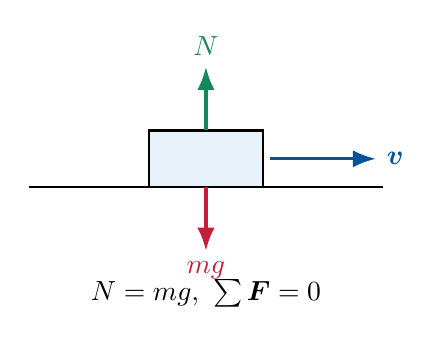
\begin{tikzpicture}[scale=0.9,>=Latex]
      \draw[thick] (-2.5,0)--(2.5,0);
      \draw[fill=SoftBlue,thick] (-0.8,0) rectangle (0.8,0.8);
      \draw[->,very thick,JapanBlue] (0.9,0.4)--(2.4,0.4)
        node[right] {$\vect v$};
      \draw[->,very thick,ForceGreen] (0,0.8)--(0,1.7)
        node[above] {$N$};
      \draw[->,very thick,ChinaRed] (0,0)--(0,-0.9)
        node[below] {$mg$};
      \node at (0,-1.5) {$N=mg,\ \sum\vect F=0$};
    \end{tikzpicture}
  \end{columns}
\end{frame}

\begin{frame}{第二法則：運動方程式}
  \begin{columns}[T,onlytextwidth]
    \column{0.52\textwidth}
    \begin{block}{ベクトル式}
      \[
        \boxed{\sum\vect F=m\vect a}
      \]
      加速度の向きは\key{合力の向き}と同じ。速度の向きとは
      必ずしも同じではない。
    \end{block}
    成分ごとに
    \[
      \sum F_x=ma_x,\qquad
      \sum F_y=ma_y.
    \]

    \column{0.44\textwidth}
    \begin{block}{解题步骤}
      \begin{enumerate}
        \item 研究对象を一つ選ぶ。
        \item その物体に働く力だけを描く。
        \item 正方向を決める。
        \item 成分ごとに式を書く。
      \end{enumerate}
    \end{block}
    \begin{alertblock}{質量と重さ}
      質量 $m$ の単位は kg。重さ $mg$ は力で、単位は N。
    \end{alertblock}
  \end{columns}
\end{frame}

\begin{frame}{第三法則：作用・反作用}
  \begin{columns}[T,onlytextwidth]
    \column{0.54\textwidth}
    物体 $A$ が $B$ に及ぼす力と、$B$ が $A$ に及ぼす力は
    \[
      \boxed{\vect F_{A\to B}=-\vect F_{B\to A}}
    \]
    \begin{itemize}
      \item 大きさが等しい。
      \item 向きが反対。
      \item 同一直線上。
      \item 同時に生じ、\key{別々の物体}に働く。
    \end{itemize}

    \column{0.42\textwidth}
    \centering
    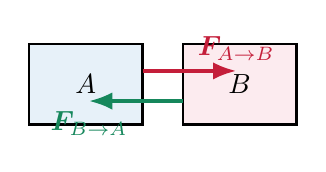
\begin{tikzpicture}[scale=0.85,>=Latex]
      \draw[fill=SoftBlue,thick] (-2,0) rectangle (-0.3,1.2);
      \draw[fill=SoftRed,thick] (0.3,0) rectangle (2,1.2);
      \node at (-1.15,0.6) {$A$};
      \node at (1.15,0.6) {$B$};
      \draw[->,very thick,ChinaRed] (-0.3,0.8)--(1.1,0.8)
        node[above] {$\vect F_{A\to B}$};
      \draw[->,very thick,ForceGreen] (0.3,0.35)--(-1.1,0.35)
        node[below] {$\vect F_{B\to A}$};
    \end{tikzpicture}
    \begin{alertblock}{平衡力とは違う}
      平衡力は\key{同じ物体}に働き、作用反作用は
      \key{異なる物体}に働く。
    \end{alertblock}
  \end{columns}
\end{frame}

\begin{frame}{例題5｜水平面上の物体：問題}
  \vfill
  \qcard{
    質量 $4.0\,\mathrm{kg}$ の物体を、水平右向きに $18\,\mathrm N$ で引く。
    動摩擦力は左向きに $6.0\,\mathrm N$ である。
    物体の加速度の大きさと向きを求めよ。
  }
  \vfill
\end{frame}

\begin{frame}{例題5｜水平面上の物体：解答}
  \qsmall{
    $m=4.0\,\mathrm{kg}$、右向き $18\,\mathrm N$、
    左向き摩擦 $6.0\,\mathrm N$。加速度を求める。
  }
  \begin{columns}[T,onlytextwidth]
    \column{0.46\textwidth}
    \centering
    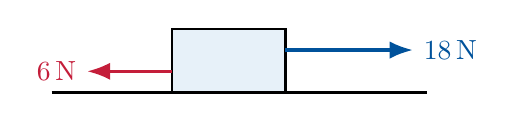
\begin{tikzpicture}[scale=0.9,>=Latex]
      \draw[thick] (-2.5,0)--(2.8,0);
      \draw[fill=SoftBlue,thick] (-0.8,0) rectangle (0.8,0.9);
      \draw[->,very thick,JapanBlue] (0.8,0.6)--(2.6,0.6)
        node[right] {$18\,\mathrm N$};
      \draw[->,very thick,ChinaRed] (-0.8,0.3)--(-2,0.3)
        node[left] {$6\,\mathrm N$};
    \end{tikzpicture}
    \column{0.50\textwidth}
    \acard{
      右向きを正とする。
      \[
        \sum F_x=18-6=12\,\mathrm N
      \]
      \[
        a=\frac{\sum F_x}{m}
        =\frac{12}{4.0}
        =\boxed{3.0\,\mathrm{m/s^2}}
      \]
      \ans{右向きに $3.0\,\mathrm{m/s^2}$。}
    }
  \end{columns}
\end{frame}

\begin{frame}{例題6｜二つの物体：問題}
  \vfill
  \qcard{
    なめらかな水平面上で、質量 $2.0\,\mathrm{kg}$ の物体 $A$ と
    $3.0\,\mathrm{kg}$ の物体 $B$ が接している。$A$ を右向きに
    $20\,\mathrm N$ で押す。二物体の加速度と、$A$ が $B$ を押す力を求めよ。
  }
  \vfill
\end{frame}

\begin{frame}{例題6｜二つの物体：解答}
  \qsmall{
    $m_A=2.0\,\mathrm{kg}$、$m_B=3.0\,\mathrm{kg}$、外力 $20\,\mathrm N$。
    加速度と接触力を求める。
  }
  \begin{columns}[T,onlytextwidth]
    \column{0.45\textwidth}
    \centering
    \begin{tikzpicture}[scale=0.85,>=Latex]
      \draw[thick] (-2.8,0)--(2.8,0);
      \draw[fill=SoftBlue,thick] (-1.5,0) rectangle (0,1);
      \draw[fill=SoftRed,thick] (0,0) rectangle (1.8,1);
      \node at (-0.75,0.5) {$A:2\,\mathrm{kg}$};
      \node at (0.9,0.5) {$B:3\,\mathrm{kg}$};
      \draw[->,very thick,JapanBlue] (-2.7,0.75)--(-1.5,0.75)
        node[midway,above] {$20\,\mathrm N$};
      \node[below] at (0,-0.25) {図の右向きを正とみなす};
    \end{tikzpicture}
    \column{0.51\textwidth}
    \acard{
      全体系について
      \[
        a=\frac{20}{2.0+3.0}=4.0\,\mathrm{m/s^2}.
      \]
      次に $B$ だけを見ると、水平力は接触力 $N$ のみ。
      \[
        N=m_Ba=3.0\times4.0=\boxed{12\,\mathrm N}.
      \]
      \ans{$a=4.0\,\mathrm{m/s^2}$、$A$ が $B$ を押す力は $12\,\mathrm N$。}
    }
  \end{columns}
\end{frame}

\begin{frame}{例題7｜エレベーター：問題}
  \vfill
  \qcard{
    質量 $50\,\mathrm{kg}$ の人がエレベーター内の体重計に乗る。
    エレベーターが上向きに $2.0\,\mathrm{m/s^2}$ で加速するとき、
    体重計の示す値（垂直抗力）を求めよ。$g=9.8\,\mathrm{m/s^2}$。
  }
  \vfill
\end{frame}

\begin{frame}{例題7｜エレベーター：解答}
  \qsmall{
    $m=50\,\mathrm{kg}$、上向き加速度 $2.0\,\mathrm{m/s^2}$。
    体重計が示す垂直抗力 $N$ は？
  }
  \begin{columns}[T,onlytextwidth]
    \column{0.40\textwidth}
    \centering
    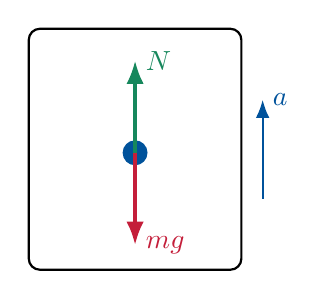
\begin{tikzpicture}[scale=0.9,>=Latex]
      \draw[rounded corners,thick] (-1.5,-1.2) rectangle (1.5,2.2);
      \fill[JapanBlue] (0,0.45) circle (5pt);
      \draw[->,very thick,ForceGreen] (0,0.45)--(0,1.75)
        node[right] {$N$};
      \draw[->,very thick,ChinaRed] (0,0.45)--(0,-0.85)
        node[right] {$mg$};
      \draw[->,thick,JapanBlue] (1.8,-0.2)--(1.8,1.2)
        node[right] {$a$};
    \end{tikzpicture}
    \column{0.56\textwidth}
    \acard{
      上向きを正とする。
      \[
        N-mg=ma
      \]
      \[
        N=m(g+a)
        =50(9.8+2.0)
        =\boxed{590\,\mathrm N}
      \]
      加速向上时，示数比静止时的 $490\,\mathrm N$ 大。
    }
  \end{columns}
\end{frame}

\begin{frame}{例題8｜作用・反作用：問題}
  \vfill
  \qcard{
    人が水平な床の上に静止している。次のうち、人に働く重力と
    作用・反作用の関係にある力はどれか。
    \begin{enumerate}
      \item 床が人を押す垂直抗力
      \item 人が床を押す力
      \item 人が地球を引く万有引力
      \item 床に働く重力
    \end{enumerate}
  }
  \vfill
\end{frame}

\begin{frame}{例題8｜作用・反作用：解答}
  \qsmall{
    人に働く重力の反作用は、垂直抗力・人が床を押す力・
    人が地球を引く力・床の重力のどれか。
  }
  \acard{
    \[
      \boxed{\text{3. 人が地球を引く万有引力}}
    \]
    人に働く重力は「地球が人を引く力」。その反作用は
    「人が地球を引く力」であり、二つは別々の物体に働く。

    \vspace{0.5em}
    垂直抗力と重力は人という\key{同じ物体}に働き、静止時には
    大きさが等しいが、これは作用・反作用ではなく\jp{平衡力}である。
  }
\end{frame}

% ============================================================
\section{仕事・仕事率}

\begin{frame}{仕事の定義}
  \begin{columns}[T,onlytextwidth]
    \column{0.52\textwidth}
    一定の力 $\vect F$ が物体を変位 $\vect s$ だけ動かしたとき
    \[
      \boxed{W=\vect F\cdot\vect s=Fs\cos\theta}
    \]
    \[
      [W]=\mathrm J=\mathrm{N\,m}
    \]
    \begin{itemize}
      \item $F\cos\theta$：変位方向の力成分。
      \item $s\cos\theta$：力方向の変位成分。
      \item 仕事は\key{スカラー量}。
    \end{itemize}
    \column{0.44\textwidth}
    \centering
    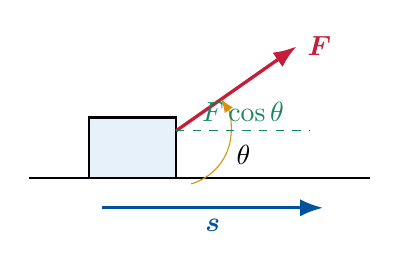
\begin{tikzpicture}[scale=0.85,>=Latex]
      \coordinate (Awork) at (0,0);
      \coordinate (Bwork) at (-0.2,0.7);
      \coordinate (Cwork) at ($(Bwork)+(35:1)$);
      \draw[thick] (-2.4,0)--(2.7,0);
      \draw[fill=SoftBlue,thick] (-1.5,0) rectangle (-0.2,0.9);
      \draw[->,very thick,ChinaRed] (-0.2,0.7)--++(35:2.2)
        node[right] {$\vect F$};
      \draw[->,very thick,JapanBlue] (-1.3,-0.45)--(2.0,-0.45)
        node[midway,below] {$\vect s$};
      \draw pic[
        draw=ForceGold,->,angle radius=7mm,
        angle eccentricity=1.3,"$\theta$"
      ]{angle=Awork--Bwork--Cwork};
      \draw[dashed,ForceGreen] (-0.2,0.7)--(1.8,0.7)
        node[midway,above] {$F\cos\theta$};
    \end{tikzpicture}
  \end{columns}
\end{frame}

\begin{frame}{正の仕事・負の仕事・仕事ゼロ}
  \begin{columns}[T,onlytextwidth]
    \column{0.31\textwidth}
    \begin{block}{正の仕事}
      $0^\circ\le\theta<90^\circ$
      \[
        W>0
      \]
      一般に速さを増やす。
    \end{block}
    \column{0.31\textwidth}
    \begin{alertblock}{負の仕事}
      $90^\circ<\theta\le180^\circ$
      \[
        W<0
      \]
      摩擦力など。
    \end{alertblock}
    \column{0.31\textwidth}
    \begin{exampleblock}{仕事ゼロ}
      $\theta=90^\circ$
      \[
        W=0
      \]
      等速円運動の向心力など。
    \end{exampleblock}
  \end{columns}

  \vfill
  \begin{block}{注意}
    力が存在するだけでは仕事とはいえない。
    \key{力の作用点が変位し、その変位方向成分がある}ときに仕事をする。
  \end{block}
\end{frame}

\begin{frame}{$F$--$x$ グラフと仕事}
  力が位置によって変化するとき、仕事はグラフの符号付き面積。
  \[
    \boxed{W=\int_{x_1}^{x_2}F_x\,dx}
  \]
  \begin{columns}[T,onlytextwidth]
    \column{0.53\textwidth}
    \centering
    \begin{tikzpicture}[x=0.9cm,y=0.42cm,>=Latex]
      \draw[->] (-0.3,0)--(5.4,0) node[right] {$x$};
      \draw[->] (0,-1.2)--(0,5.5) node[above] {$F_x$};
      \fill[SoftBlue] (0,0)--(2,4)--(4,4)--(5,0)--cycle;
      \draw[very thick,JapanBlue] (0,0)--(2,4)--(4,4)--(5,0);
      \draw[dashed] (2,0)--(2,4) (4,0)--(4,4);
      \node[JapanBlue] at (2.6,2.0) {面積 $=W$};
    \end{tikzpicture}
    \column{0.43\textwidth}
    \begin{itemize}
      \item $x$ 軸より上：正の仕事。
      \item $x$ 軸より下：負の仕事。
      \item 長方形・三角形・台形に分けると EJU で計算しやすい。
    \end{itemize}
  \end{columns}
\end{frame}

\begin{frame}{仕事率（しごとりつ）}
  \begin{columns}[T,onlytextwidth]
    \column{0.52\textwidth}
    \begin{block}{平均の仕事率 \en{average power}}
      \[
        \boxed{\overline P=\frac{W}{\Delta t}}
      \]
    \end{block}
    \begin{block}{瞬間の仕事率 \en{instantaneous power}}
      \[
        \boxed{P=\frac{dW}{dt}=\vect F\cdot\vect v
        =Fv\cos\theta}
      \]
    \end{block}
    \[
      [P]=\mathrm W=\mathrm{J/s}
    \]
    \column{0.44\textwidth}
    \begin{alertblock}{功率不等于功}
      功描述能量转移的总量；功率描述转移的快慢。
      做功相同，用时越短，功率越大。
    \end{alertblock}
    \begin{block}{効率}
      \[
        \eta=\frac{\text{有効な出力}}{\text{入力}}\times100\%
      \]
    \end{block}
  \end{columns}
\end{frame}

\begin{frame}{例題9｜斜めに引く：問題}
  \vfill
  \qcard{
    水平面上の物体を、水平となす角 $60^\circ$ の方向に
    $40\,\mathrm N$ の一定力で引き、水平に $5.0\,\mathrm m$ 移動させた。
    この力のした仕事を求めよ。
  }
  \vfill
\end{frame}

\begin{frame}{例題9｜斜めに引く：解答}
  \qsmall{
    $F=40\,\mathrm N$、$s=5.0\,\mathrm m$、力と変位の角は $60^\circ$。
    この力の仕事を求める。
  }
  \acard{
    \[
      W=Fs\cos\theta
      =40\times5.0\times\cos60^\circ
      =\boxed{100\,\mathrm J}
    \]
    铅直方向分量与水平位移垂直，因此不做功。
  }
\end{frame}

\begin{frame}{例題10｜摩擦力の仕事：問題}
  \vfill
  \qcard{
    質量 $2.0\,\mathrm{kg}$ の物体が粗い水平面を $8.0\,\mathrm m$ 滑る。
    動摩擦係数は $0.25$ である。$g=10\,\mathrm{m/s^2}$ として、
    重力・垂直抗力・動摩擦力のした仕事をそれぞれ求めよ。
  }
  \vfill
\end{frame}

\begin{frame}{例題10｜摩擦力の仕事：解答}
  \qsmall{
    $m=2.0\,\mathrm{kg}$、$\mu'=0.25$、水平距離 $8.0\,\mathrm m$。
    重力・垂直抗力・摩擦力の仕事を求める。
  }
  \acard{
    水平面なので $N=mg=20\,\mathrm N$、
    \[
      f=\mu'N=0.25\times20=5.0\,\mathrm N.
    \]
    重力と垂直抗力は変位に垂直：
    \[
      \boxed{W_g=0,\qquad W_N=0}.
    \]
    摩擦力は変位と反対：
    \[
      W_f=-fs=-5.0\times8.0=\boxed{-40\,\mathrm J}.
    \]
  }
\end{frame}

\begin{frame}{例題11｜$F$--$x$ グラフ：問題}
  \begin{columns}[T,onlytextwidth]
    \column{0.52\textwidth}
    \qcard{
      右図のように、力 $F_x$ が位置 $x$ によって変化する。
      $x=0$ から $6.0\,\mathrm m$ までにこの力がした仕事を求めよ。
    }
    \column{0.44\textwidth}
    \centering
    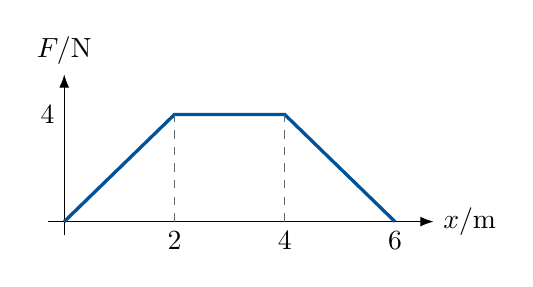
\begin{tikzpicture}[x=0.7cm,y=0.34cm,>=Latex]
      \draw[->] (-0.3,0)--(6.7,0) node[right] {$x/\mathrm m$};
      \draw[->] (0,-0.5)--(0,5.5) node[above] {$F/\mathrm N$};
      \draw[very thick,JapanBlue] (0,0)--(2,4)--(4,4)--(6,0);
      \draw[dashed,GraphGray] (2,0)--(2,4) (4,0)--(4,4);
      \foreach \x in {2,4,6}
        \node[below] at (\x,0) {\x};
      \node[left] at (0,4) {4};
    \end{tikzpicture}
  \end{columns}
\end{frame}

\begin{frame}{例題11｜$F$--$x$ グラフ：解答}
  \qsmall{
    $F$ は $0$--$2\,\mathrm m$ で $0$ から $4\,\mathrm N$、
    $2$--$4\,\mathrm m$ で $4\,\mathrm N$、
    $4$--$6\,\mathrm m$ で $4$ から $0\,\mathrm N$。
  }
  \acard{
    グラフ下の面積を、三角形＋長方形＋三角形に分ける。
    \[
      W=
      \frac12(2)(4)+(2)(4)+\frac12(2)(4)
      =4+8+4
      =\boxed{16\,\mathrm J}
    \]
  }
\end{frame}

\begin{frame}{例題12｜エレベーターの出力：問題}
  \vfill
  \qcard{
    総質量 $800\,\mathrm{kg}$ のエレベーターを、一定の速さ
    $2.5\,\mathrm{m/s}$ で上昇させる。摩擦を無視し、
    $g=9.8\,\mathrm{m/s^2}$ とする。モーターの出力を求めよ。
  }
  \vfill
\end{frame}

\begin{frame}{例題12｜エレベーターの出力：解答}
  \qsmall{
    $m=800\,\mathrm{kg}$、一定速度 $v=2.5\,\mathrm{m/s}$ で上昇。
    摩擦なし。必要な出力は？
  }
  \acard{
    等速なのでモーターの力は重力と等しい：
    \[
      F=mg=800\times9.8=7840\,\mathrm N.
    \]
    力と速度は同方向なので
    \[
      P=Fv=7840\times2.5
      =1.96\times10^4\,\mathrm W
      =\boxed{19.6\,\mathrm{kW}}.
    \]
  }
\end{frame}

% ============================================================
\section{力学的エネルギーと保存則}

\begin{frame}{三つの基本エネルギー}
  \begin{columns}[T,onlytextwidth]
    \column{0.31\textwidth}
    \begin{block}{運動エネルギー}
      \[
        \boxed{K=\frac12mv^2}
      \]
      速さにより決まる。
    \end{block}
    \column{0.31\textwidth}
    \begin{block}{重力による位置}
      \[
        \boxed{U_g=mgh}
      \]
      基準面からの高さ。
    \end{block}
    \column{0.31\textwidth}
    \begin{block}{弾性エネルギー}
      \[
        \boxed{U_s=\frac12kx^2}
      \]
      ばねの自然長からの変形。
    \end{block}
  \end{columns}

  \vfill
  \begin{alertblock}{位置エネルギーの基準}
    $U=0$ の位置は自由に選べる。物理的に意味があるのは
    \key{位置エネルギーの差} $\Delta U$。
  \end{alertblock}
\end{frame}

\begin{frame}{仕事と運動エネルギー}
  \begin{block}{仕事と運動エネルギーの関係}
    物体に働く\key{合力の仕事}は、運動エネルギーの変化に等しい。
    \[
      \boxed{W_{\mathrm{net}}=\Delta K
      =\frac12mv_2^2-\frac12mv_1^2}
    \]
  \end{block}

  \begin{columns}[T,onlytextwidth]
    \column{0.46\textwidth}
    \begin{itemize}
      \item $W_{\mathrm{net}}>0$：速くなる。
      \item $W_{\mathrm{net}}<0$：遅くなる。
      \item $W_{\mathrm{net}}=0$：速さは不変。
    \end{itemize}
    \column{0.50\textwidth}
    \begin{alertblock}{方向には直接答えない}
      $K$ はスカラーで速さだけを含む。
      速度方向を求める問題では、運動方程式や運動学も併用する。
    \end{alertblock}
  \end{columns}
\end{frame}

\begin{frame}{保存力と力学的エネルギー}
  \begin{columns}[T,onlytextwidth]
    \column{0.50\textwidth}
    \begin{block}{保存力（ほぞんりょく）}
      仕事が経路によらず、始点と終点だけで決まる力。
      \[
        W_c=-\Delta U
      \]
      例：重力、弾性力、万有引力。
    \end{block}
    \column{0.46\textwidth}
    \begin{block}{非保存力}
      仕事が経路に依存する力。
      例：動摩擦力、空気抵抗。
    \end{block}
    \begin{alertblock}{重要}
      垂直抗力は仕事 0 になることが多いが、
      「仕事 0」と「保存力」は同じ意味ではない。
    \end{alertblock}
  \end{columns}
\end{frame}

\begin{frame}{力学的エネルギー保存則}
  \begin{block}{保存力だけが仕事をする場合}
    \[
      \boxed{E=K+U=\text{一定}}
    \]
    \[
      \boxed{K_1+U_1=K_2+U_2}
    \]
  \end{block}

  \begin{columns}[T,onlytextwidth]
    \column{0.48\textwidth}
    \centering
    \begin{tikzpicture}[x=0.9cm,y=0.25cm]
      \draw[thick] (0,0) rectangle (1.1,8);
      \fill[JapanBlue] (0,0) rectangle (1.1,2);
      \fill[ForceGold] (0,2) rectangle (1.1,8);
      \node at (0.55,-0.8) {高い位置};
      \node[white] at (0.55,1) {$K$};
      \node at (0.55,5) {$U$};
      \draw[thick] (2.2,0) rectangle (3.3,8);
      \fill[JapanBlue] (2.2,0) rectangle (3.3,6.3);
      \fill[ForceGold] (2.2,6.3) rectangle (3.3,8);
      \node at (2.75,-0.8) {低い位置};
      \node[white] at (2.75,3.1) {$K$};
      \node at (2.75,7.15) {$U$};
    \end{tikzpicture}
    \column{0.48\textwidth}
    \begin{itemize}
      \item 落下：$U_g$ が減り、$K$ が増える。
      \item ばね：$U_s$ と $K$ が相互変換。
      \item 机械能不是“消失”，而是在各种形式间转化。
    \end{itemize}
  \end{columns}
\end{frame}

\begin{frame}{摩擦があるとき：一般化したエネルギー式}
  \begin{block}{非保存力の仕事}
    \[
      \boxed{W_{\mathrm{nc}}=\Delta(K+U)}
    \]
    すなわち
    \[
      \boxed{K_1+U_1+W_{\mathrm{nc}}=K_2+U_2}.
    \]
  \end{block}

  動摩擦力が一定なら
  \[
    W_f=-fs=-\mu'Ns.
  \]
  失われた力学的エネルギーは主に内部エネルギー（熱）へ変わる。

  \vfill
  \begin{alertblock}{よくある誤り}
    摩擦があるのに $K_1+U_1=K_2+U_2$ と書かない。
    先に\key{系の境界}と\key{保存則の成立条件}を確認する。
  \end{alertblock}
\end{frame}

\begin{frame}{例題13｜自由落下：問題}
  \vfill
  \qcard{
    質量 $2.0\,\mathrm{kg}$ の物体を地面から高さ $20\,\mathrm m$ の位置で
    静かに放す。空気抵抗を無視し、$g=9.8\,\mathrm{m/s^2}$ とする。
    地面に達する直前の速さを、力学的エネルギー保存則で求めよ。
  }
  \vfill
\end{frame}

\begin{frame}{例題13｜自由落下：解答}
  \qsmall{
    高さ $20\,\mathrm m$ から静かに放す。空気抵抗なし。
    地面直前の速さを求める。
  }
  \acard{
    地面を $U=0$ とする。初めは $v_1=0$。
    \[
      mgh=\frac12mv^2
    \]
    質量 $m$ は消去され、
    \[
      v=\sqrt{2gh}
      =\sqrt{2\times9.8\times20}
      \approx\boxed{19.8\,\mathrm{m/s}}.
    \]
    同じ高さから落とせば、空気抵抗なしでは質量によらず同じ速さ。
  }
\end{frame}

\begin{frame}{例題14｜ばねによる発射：問題}
  \vfill
  \qcard{
    ばね定数 $k=200\,\mathrm{N/m}$ の軽いばねを $0.10\,\mathrm m$ 縮め、
    質量 $0.50\,\mathrm{kg}$ の物体をなめらかな水平面上で静かに放す。
    ばねが自然長になった瞬間の物体の速さを求めよ。
  }
  \vfill
\end{frame}

\begin{frame}{例題14｜ばねによる発射：解答}
  \qsmall{
    $k=200\,\mathrm{N/m}$、圧縮 $x=0.10\,\mathrm m$、
    $m=0.50\,\mathrm{kg}$。自然長での速さを求める。
  }
  \begin{columns}[T,onlytextwidth]
    \column{0.44\textwidth}
    \centering
    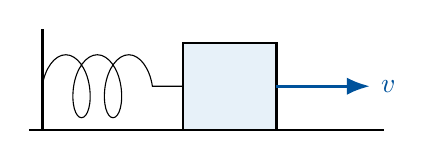
\begin{tikzpicture}[scale=0.85,>=Latex]
      \draw[thick] (-2.6,0)--(2.7,0);
      \draw[very thick] (-2.4,0)--(-2.4,1.5);
      \draw[decorate,decoration={coil,aspect=0.5,segment length=4mm,amplitude=4mm}]
        (-2.4,0.65)--(-0.3,0.65);
      \draw[fill=SoftBlue,thick] (-0.3,0) rectangle (1.1,1.3);
      \draw[->,very thick,JapanBlue] (1.1,0.65)--(2.5,0.65)
        node[right] {$v$};
    \end{tikzpicture}
    \column{0.52\textwidth}
    \acard{
      ばねの弾性エネルギーが運動エネルギーへ変わる。
      \[
        \frac12kx^2=\frac12mv^2
      \]
      \[
        v=x\sqrt{\frac{k}{m}}
        =0.10\sqrt{\frac{200}{0.50}}
        =\boxed{2.0\,\mathrm{m/s}}.
      \]
    }
  \end{columns}
\end{frame}

\begin{frame}{例題15｜粗い斜面：問題}
  \vfill
  \qcard{
    質量 $2.0\,\mathrm{kg}$ の物体を、高さ $5.0\,\mathrm m$ の斜面上端から
    静かに滑らせる。斜面を下る間に摩擦力がした仕事は
    $-20\,\mathrm J$ であった。$g=10\,\mathrm{m/s^2}$ として、
    下端での速さを求めよ。
  }
  \vfill
\end{frame}

\begin{frame}{例題15｜粗い斜面：解答}
  \qsmall{
    $m=2.0\,\mathrm{kg}$、$h=5.0\,\mathrm m$、$W_f=-20\,\mathrm J$。
    静止から滑り、下端の速さを求める。
  }
  \acard{
    下端を $U=0$ として
    \[
      K_1+U_1+W_f=K_2+U_2.
    \]
    \[
      0+(2.0)(10)(5.0)-20
      =\frac12(2.0)v^2.
    \]
    \[
      80=v^2
      \quad\Rightarrow\quad
      v=\sqrt{80}\approx\boxed{8.9\,\mathrm{m/s}}.
    \]
  }
\end{frame}

\begin{frame}{例題16｜振り子：問題}
  \vfill
  \qcard{
    長さ $L$ の糸につけた小球を、最下点より高さ $h$ の位置から
    静かに放す。空気抵抗を無視する。小球が最下点を通過するときの
    速さ $v$ を求めよ。また、質量に依存するか。
  }
  \vfill
\end{frame}

\begin{frame}{例題16｜振り子：解答}
  \qsmall{
    最下点より高さ $h$ から静かに放した振り子。
    最下点の速さと質量依存性を求める。
  }
  \begin{columns}[T,onlytextwidth]
    \column{0.40\textwidth}
    \centering
    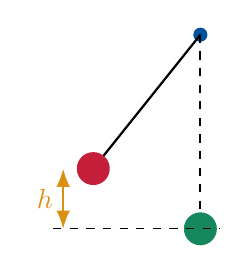
\begin{tikzpicture}[scale=0.85,>=Latex]
      \fill[JapanBlue] (0,2.8) circle (3pt);
      \draw[thick] (0,2.8)--(-1.6,0.8);
      \draw[thick,dashed] (0,2.8)--(0,-0.1);
      \fill[ChinaRed] (-1.6,0.8) circle (7pt);
      \fill[ForceGreen] (0,-0.1) circle (7pt);
      \draw[<->,ForceGold,thick] (-2.05,-0.1)--(-2.05,0.8)
        node[midway,left] {$h$};
      \draw[dashed] (-2.2,-0.1)--(0.3,-0.1);
    \end{tikzpicture}
    \column{0.56\textwidth}
    \acard{
      最下点を $U=0$ とする。
      \[
        mgh=\frac12mv^2
      \]
      \[
        \boxed{v=\sqrt{2gh}}
      \]
      質量は消去されるので、\key{質量には依存しない}。
      张力始终与瞬时位移垂直，因此不做功。
    }
  \end{columns}
\end{frame}

\begin{frame}{例題17｜仕事率とエネルギー：問題}
  \vfill
  \qcard{
    出力 $1.5\,\mathrm{kW}$ のモーターで、質量 $100\,\mathrm{kg}$ の荷物を
    一定速度で鉛直上方へ運ぶ。損失を無視し、$g=10\,\mathrm{m/s^2}$ とする。
    20 秒間に荷物は何 m 上昇するか。
  }
  \vfill
\end{frame}

\begin{frame}{例題17｜仕事率とエネルギー：解答}
  \qsmall{
    $P=1.5\,\mathrm{kW}$、$m=100\,\mathrm{kg}$、一定速度。
    20 秒間の上昇距離を求める。
  }
  \acard{
    20 秒間にモーターがした仕事は
    \[
      W=Pt=1500\times20=3.0\times10^4\,\mathrm J.
    \]
    一定速度なので運動エネルギーは変化せず、仕事は位置エネルギーへ：
    \[
      mgh=W.
    \]
    \[
      h=\frac{3.0\times10^4}{100\times10}
      =\boxed{30\,\mathrm m}.
    \]
  }
\end{frame}

\begin{frame}{発展：保存則と運動方程式の使い分け}
  \begin{tabular}{>{\bfseries\color{JapanBlue}}p{0.22\linewidth}p{0.31\linewidth}p{0.37\linewidth}}
    方法 & 得意な問題 & 注意点\\
    \toprule
    運動方程式 &
    力・加速度・張力・垂直抗力を求める &
    ベクトルなので方向と成分が必要\\[0.7em]
    運動学公式 &
    等加速度運動の時間・変位・速度 &
    加速度が一定か確認\\[0.7em]
    エネルギー &
    始点と終点の速さ・高さ・ばね変形 &
    時間や方向は直接出ない\\[0.7em]
    運動量保存 &
    衝突・爆発・短時間の相互作用 &
    系への外力積を確認
  \end{tabular}

  \vfill
  \begin{block}{選び方}
    求めたい量を見て、一番短い法則を選ぶ。
    必要なら複数の法則を段階的に組み合わせる。
  \end{block}
\end{frame}

% ============================================================
\section{まとめ・確認問題}

\begin{frame}{重要語彙}
  \small
  \begin{tabular}{p{0.25\linewidth}p{0.29\linewidth}p{0.34\linewidth}}
    \toprule
    日本語 & 読み方 & 中文・English\\
    \midrule
    剛体 & ごうたい & 刚体 / rigid body\\
    力のモーメント & ちからのモーメント & 力矩 / torque\\
    腕の長さ & うでのながさ & 力臂 / lever arm\\
    支点 & してん & 支点 / pivot\\
    重心 & じゅうしん & 重心 / center of gravity\\
    慣性 & かんせい & 惯性 / inertia\\
    運動方程式 & うんどうほうていしき & 运动方程\\
    作用・反作用 & さよう・はんさよう & 作用与反作用\\
    仕事 & しごと & 功 / work\\
    仕事率 & しごとりつ & 功率 / power\\
    運動エネルギー & うんどうエネルギー & 动能\\
    位置エネルギー & いちエネルギー & 势能\\
    保存力 & ほぞんりょく & 保守力\\
    力学的エネルギー & りきがくてきエネルギー & 机械能\\
    \bottomrule
  \end{tabular}
\end{frame}

\begin{frame}{公式マップ}
  \begin{columns}[T,onlytextwidth]
    \column{0.48\textwidth}
    \begin{block}{力・回転}
      \[
        \tau=rF\sin\theta=Fd
      \]
      \[
        \sum\vect F=0,\qquad \sum\tau=0
      \]
      \[
        \sum\vect F=m\vect a
      \]
    \end{block}
    \begin{block}{ニュートン第三法則}
      \[
        \vect F_{A\to B}=-\vect F_{B\to A}
      \]
    \end{block}
    \column{0.48\textwidth}
    \begin{block}{仕事・仕事率}
      \[
        W=Fs\cos\theta,\qquad P=\frac Wt=\vect F\cdot\vect v
      \]
    \end{block}
    \begin{block}{エネルギー}
      \[
        K=\frac12mv^2,\quad U_g=mgh,\quad U_s=\frac12kx^2
      \]
      \[
        W_{\rm net}=\Delta K,\qquad
        W_{\rm nc}=\Delta(K+U)
      \]
    \end{block}
  \end{columns}
\end{frame}

\begin{frame}{授業内確認問題：問題}
  \qcard{
    次の記述の正誤を判断し、誤りなら訂正せよ。
    \begin{enumerate}
      \item 物体が静止していれば、その物体に力は働いていない。
      \item 作用・反作用の二力は、同じ物体に働いてつり合う。
      \item 力が変位に垂直なら、その力の仕事は 0 である。
      \item 摩擦が働く場合、力学的エネルギーは必ず保存する。
      \item 剛体が静止するには、合力が 0 だけで十分である。
    \end{enumerate}
  }
\end{frame}

\begin{frame}{授業内確認問題：解答}
  \qsmall{
    静止と力、作用反作用、垂直な力の仕事、摩擦と機械エネルギー、
    剛体の静止条件について正誤を判断する。
  }
  \acard{
    \begin{enumerate}
      \item \key{誤}。静止は合力が 0 という意味で、複数の力が働くことがある。
      \item \key{誤}。作用・反作用は別々の物体に働く。
      \item \jp{正}。$W=Fs\cos90^\circ=0$。
      \item \key{誤}。摩擦の仕事を含めてエネルギー式を書く。
      \item \key{誤}。$\sum\vect F=0$ と $\sum\tau=0$ の両方が必要。
    \end{enumerate}
  }
\end{frame}

\begin{frame}{宿題}
  \begin{enumerate}
    \item 一様な棒と荷重について、支持力を求める問題を 2 題。
    \item 二物体連結系について、加速度と接触力・張力を求める問題を 3 題。
    \item $F$--$x$ グラフの面積から仕事を求める問題を 2 題。
    \item 斜面・ばね・自由落下について、エネルギー法で解く問題を各 1 題。
  \end{enumerate}

  \vfill
  \begin{alertblock}{书写要求}
    每题必须包含：研究对象、受力图或能量状态图、所用定律、带单位的答案。
    只写最后结果不计完整过程。
  \end{alertblock}
\end{frame}

\begin{frame}[plain]
  \vfill
  \centering
  {\Huge\color{JapanBlue}\bfseries お疲れさまでした！}

  \vspace{1.2em}
  {\Large 次回：運動量・力積・衝突}
  \vfill
\end{frame}

\end{document}
